\chapter{Introduction} \label{Chapter:introduction}

%\begin{enumerate}
%\item Introduction to comp chem
%\item Why is it important to calculate interactions between molecules (drug discovery etc..)
%\item Why we use free energies (Exp comparison)
%\item How free energies are currently calculated (Classical mechanics)
%\item Correcting free energies QM/MM, using full QM etc..
%\item Desired free energies (using ab initio MD)
%\end{enumerate}

Since the discovery of classical mechanics by Isaac Newton, models and theories have been used to explain natural phenomena.  It wasn't until the early 1900's that physicists discovered that classical mechanics cannot accurately describe the behaviour of small particles and the rules of quantum mechanics were developed.  Since then, chemists have applied these rules to try and explain and/or predict experimental results.  The recent rise in popularity of using these theoretical models is largely down to the lowering cost of computational resources and the large leaps forward in technological development in the last few decades.

Pharmaceutical companies use computational chemical methods to predict interactions between proteins and ligands before potentially expensive experimental techniques are performed.  Because of this, it is crucial to have accurate information, as such any method is tested extensively against ``test'' systems (systems with known experimental results).  In the case of protein-ligand binding, free energies are used to compare theoretical with experimental results.  The reason for this that the experimental observable $K$ can be easily converted to the free energy $\Delta G$, which can be calculated using statistical mechanics \cite{protein-ligand_interactions_book}. $K$ is known as the association constant and is defined as,

\begin{equation}
\ K=\frac{[AB]}{[A][B]} \\.
\end{equation}

Where [] represents the concentration.  The free energy can be calculated using the following equation,

\begin{equation}
\ \Delta G_{bind} = -k_B T \ln K \\.
\end{equation}


It is clear to see that the calculation of accurate free energies of binding is crucial to the pharmaceutical industry.  The traditional method to calculate these free energies is to use classical mechanics to describe the system in combination with molecular dynamics (MD) and/or Monte Carlo (MC) to generate structures \cite{jorgensen_free_energy_review, kollman_free_energy_review}.  Enough structures are needed to satisfy the ergodic hypothesis, which simply states that the generated ensemble of structures must be a representative sample of the entire phase space \cite{jensen_quantum}.  Because free energies require a large amount of sampling to converge\cite{kollman_free_energy_review}, classical mechanics is the obvious choice due to the lower computational cost associated with it.  This approach relies on the transferability of force fields \cite{Leach_chem}, and cannot possibly model every interaction relevant to calculate accurate binding free energies.  For example, classical mechanics does not calculate charge transfer, polarisation or the exchange energy.  In standard force fields, such as the AMBER force field \cite{ff99}, the polarisation is included implicitly within the parameterisation \cite{polarisable_force_field_russian}.  However, these force fields cannot show the dependence of the electronic structure of a molecule to its environment \cite{polarisable_force_field_protein_study}.  This has led to the development of force fields that can explicitly calculate polarisation, known as polarisable force fields.  Polarisation is taken into account within these force fields by an additional term within the functional form, $U_{ele}^{ind}$ \cite{protein-ligand_interactions_book}.  The interactive induction scheme for example, will calculate the effect the surrounding electrostatics has on a polarisable site, forming a new dipole, then the effect the this dipole has on the surroundings, and repeats until convergence \cite{Simulate_Phys_world}.  This process can become computationally expensive and still provides no solution to other non-classical interactions.


Ideally, the ensemble of structures generated would be as a result of \textit{ab initio} molecular dynamics, but this is far too computationally expensive to be feasible.  This leads to the use of hybrid methods and guiding potentials.  QM/MM is an example of a hybrid method and was first suggested by Warshel et al.\cite{warhsel_qm-mm}, which is the combination of using QM for a small region of interest and MM for the surroundings.  The Hamiltonian then becomes,

\begin{equation}
\ H_{QM/MM} = E_{QM}+E_{MM}+E_{QM-MM} \\.
\end{equation}

Where $E_{QM}$ is the quantum potential energy of the region of interest, $E_{MM}$ is the potential energy of the surroundings and $E_{QM-MM}$ is the interaction of the two regions.  Some sources suggest that this is all that is needed to accurately describe interactions within protein-ligand systems, as the electron correlation is primarily short-range \cite{protein-ligand_interactions_book}.  But this still relies heavily on the forcefield to describe interactions accurately.  Difficulties arise when the QM region is bonded covalently to the MM region and a great deal of expertise is required to perform calculations using these hybrid methods \cite{cramer_chem}.  The implementation of QM/MM can be described by two categories: mechanical embedding and electrostatic embedding \cite{qm-mm_error_analysis}.  The former uses the classical force field to describe electrostatics and dispersion and the latter calculates the electrostatics and polarisation at a QM level.  The latter of the two being the more accurate \cite{eel_embed_vs_mech_embed}.

The use of a guiding potential is another common way to obtain accurate free energies, these involve using a cheap potential to sample structures, then a perturbation to a more expensive potential.  This approach uses the extended thermodynamic cycle introduced by \u{S}trajbl et al. \cite{Warshel_free_energy_correction}, which can be seen in figure \ref{fig:extended_thermodynamic_cycle}.  

\begin{center}
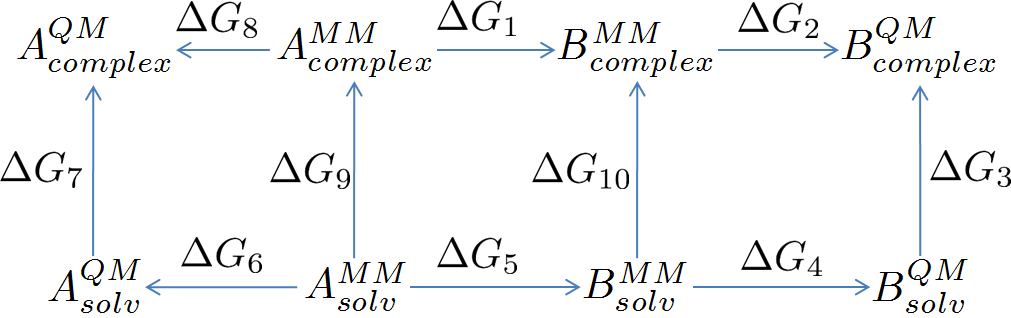
\includegraphics[width=15cm]{extended_thermodynamic_cycle.png}
 \captionof{figure}{The extended thermodynamic cycle}\label{fig:extended_thermodynamic_cycle}
\end{center}  

In this cycle, $\Delta G_1$ and $\Delta G_5$ are classical alchemical mutations of the ligand when bound in a protein and when in solvent respectively.  $\Delta G_2$, $\Delta G_4$, $\Delta G_6$ and $\Delta G_8$ are the perturbations from a classical system to a quantum system.  $\Delta G_7$ and $\Delta G_3$ are the desired free energies, but are much too computationally expensive to calculate.  However, with all the other free energies, the relative free energy ($\Delta G_7-\Delta G_3$) can be calculated by $\Delta G_1 + \Delta G_2 - \Delta G_4 - \Delta G_5 + \Delta G_6 - \Delta G_8$.

Application of the extended thermodynamic cycle has seen many uses, from reaction mechanisms \cite{Warshel_free_energy_correction, ryde_qm-mm_extended_td} to correcting binding free energies \cite{essex_qmmm, fox_mm_to_qm, mullholland_qmmm}  For the purposes of this thesis, the application will be directed toward correcting binding free energies.  Beierlein et al. \cite{essex_qmmm} correct the binding free energy using the Coulomb energies in a single step perturbation from the classical potential to a QM/MM potential.  Fox et al. \cite{fox_mm_to_qm} performed a similar task on the solvation free energies using the interaction energies this time perturbing from the classical to a fully quantum potential.  In both studies the Zwanzig equation \cite{zwanzig} was used (equation \ref{eq:Zwanzig}), however, although convergence was achieved by using interaction energies, this equation requires the use of total energies.  

\begin{equation} \label{eq:Zwanzig}
\ \Delta G = -k_B T \ln \left\langle \exp \left[ - \frac{E_{MM} - E_{QM}}{k_B T}  \right] \right\rangle
\end{equation}

Where $E_{MM}$ is the classical potential energy and $E_{QM}$ is the quantum potential energy, when interaction energies are used, these become $\Delta E_{MM}$ and $\Delta E_{QM}$.  Interaction energies can simply be described by the following,

\begin{equation}
\ E= E_{complex}-E_{ligand}-E_{host} \\.
\end{equation}

This cancels out any intramolecular terms and intermolecular interactions within the host.  The complex is the entire system e.g. a ligand bound to a protein, and within this example the host would be the protein in the same geometry but without the ligand present.  This makes the approximation that this conformation of the protein would be sampled in the absence of the ligand.  Although an approximation, it is an approximation that can provide converged free energies \cite{essex_qmmm, fox_mm_to_qm}.  One potential issue of using total energies is the overlap of configurational space.  However, Woods et al. \cite{mullholland_qmmm} have come up with a method that allows the perturbation from a classical system to a QM/MM system with the use of total energies.  Doing this involved evaluating whether a classically obtained snapshot was a good representation at the QM/MM level and accepting or rejecting it.

The search for a method that can provide accurate free energies of binding that is relatively inexpensive is one of the main challenges within computational chemistry.  As such, within this thesis, we would like to explore the possibilities of finding a method that can accurately calculate quantum corrected free energies for a range of systems when using total energy approaches.


%Chapter 1 introduction?
%Fox et al. \cite{fox_MM_to_QM} provides a brief description of the issues associated with using total energies, namely that the large size difference between the classical and quantum energies makes the calculation of the exponential numerically unstable and that there may be an issue with convergence of free energies obtained when using total energies.  